\documentclass{article}

\usepackage[final]{nips_2017}

\usepackage[utf8]{inputenc} % allow utf-8 input
\usepackage[T1]{fontenc}    % use 8-bit T1 fonts
\usepackage{hyperref}       % hyperlinks
\usepackage{url}            % simple URL typesetting
\usepackage{booktabs}       % professional-quality tables
\usepackage{amsfonts}       % blackboard math symbols
\usepackage{nicefrac}       % compact symbols for 1/2, etc.
\usepackage{microtype}      % microtypography
\usepackage{graphicx}
\usepackage{amsmath}
\usepackage{amssymb}
\usepackage{listings}
\usepackage{courier}
\usepackage{multirow}

\lstset{basicstyle=\ttfamily\footnotesize,breaklines=true}
\title{CSE 253 Programming Assignment 4 -- Generating Music with Recurrent Networks}

\author{
  Fanjin Zeng \\
  Computer Science and Engineering\\
  University of Califorina, San Diego\\
  \texttt{f1zeng@ucsd.edu} \\
   \And
   Xinyue Ou \\
   Computer Science and Engineering\\
   University of Califorina, San Diego \\
   \texttt{x1ou@ucsd.edu} \\
   \And
   He Qin \\
   Computer Science and Engineering\\
   University of Califorina, San Diego \\
   \texttt{h9qin@ucsd.edu} \\
   \And
   Yuhan Chen \\
   Eletrical and Computer Engineering\\
   University of Califorina, San Diego \\
   \texttt{yuc143@ucsd.edu} \\
}

\begin{document}

\maketitle
\begin{abstract}

\end{abstract}

\section{Music Generation}
\subsection{Music Sample}
After training the model with the whole batch of data for 7 epochs, we start to use the model we get to generate music samples. The process is as follows. First, with the hidden state re-initialize, we feed the model with a small clip of one sequence from the validation set, and update the hidden state to the last character that sequence. Then feed the last character into the model again, and generate the output, which is used as the next input. Henceforth, we get a sequence of data that starts with the pre-given small sequence clip and ends when the specified maximum character limit is reached. 

During the training, the temperature is set to be 1. For the generation phase, we produce 6 clips of music that have different temperatures: 0.5, 1, 1.5. We also try with temperature being 2, but it does not give us any sensible result. 
\newpage
\subsubsection{Temperature = 0.5}
Sample 1
\begin{lstlisting}
X:16
T:Ban
R:air at ancar he Aiso pamlasc
R:air
O:Ban pabhance
R:d tollan (1617-108)
Z:id:hn-air-18
M:4/4
L:1/8
L:1/8
K:D
G2 A2 G2 | G2 G2 D2 || G2E F2 | GE FE | G2G G2 | G2 A2 AG | G2 F2 G2 |: AB B2 |
G2 G/A/ G2 | G2 A2 AA | A2 AG A2 | G3 E2 | A4 G | G2G G2 ||
|: G>G G>A | G2 G2 G2 G2 :|
\end{lstlisting}
Sample 2
\begin{lstlisting}
X:14
T:Aranle an (Thance
R:ais-rition mareld 1 2
Z:id:hn-air-16
M:6/4
L:1/8
K:G
c2 B2 |
G2 A2 A2 | A2A A2 | G2 G2 A2 | D2 G2 C2 | G6 |: G2 E>G | AB d>c | d2 B2 cA |
A/B/A/ A2 | G2 G> F2 | G2E G2 | A2 B>B | G2 A2 A/A/ | G2 A2 AB | B2 AA E4 | G3
B2 |
G2 G2 E/2 A/B/ | c2 G3  A>G A2 | A/B/A/ G2 | A3 G2 A2 | G2 G2 F2 | D>G GG | d2
B3 c2 | A2 F2 D2 | G3 E2 | G2 G2 F2 C2 | GA E2 | A2 G2 G2 A2 | G2 A2 FA | A2 A2
B2 | E2 AB A2 | G2 A2 A2 | G6 ||
\end{lstlisting}


\begin{figure}[h]
\begin{minipage}{0.48\textwidth}
\centering
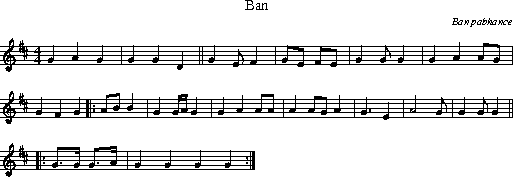
\includegraphics[width=\textwidth]{pics/generated_music_t05_1.png}
\caption{Generated sample 1 with Temperature = 0.5}
\end{minipage}\hfill
\begin{minipage}{0.48\textwidth}
\centering
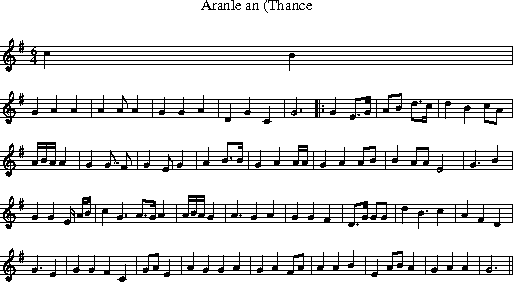
\includegraphics[width=\textwidth]{pics/generated_music_t05_2.png}
\caption{Generated sample 2 with Temperature = 0.5}
\end{minipage}
\end{figure}
\newpage
\subsubsection{Temperature = 1}
Sample 1
\begin{lstlisting}
X:1
T: Liu tote obdariel and
R:aise
arand tham Oem"LON Geanlais O'Deirle \'O. Cehssinau
C:Th Gabas Mel
R:aimbamminll Limammay
A:Sre hon Sto Asten Oe"MDyatris Rost, The Gimmia bisoiphsco? nataian
T:Bince
R:on bonsa-r
R:d:hr- be-ligd
Z:id:hansoaptoit a ewmourd Rellgc.
C:Bokle
Z:id:hn-par0-09
M:1/4
L:1/8
K:G
n:mabs
cdef e3 eG cdc | A2 :|
|: d f=fe | e2fg ddB | c2d cB | G2 G>A B>A|cBAA | B2c Ad cB|c2 d2:|
P:Varieqlanf6 :: 1
|: D2G F>E | G4 F2 | G3 G3 |A3 GAGG | G4 :|
V:rriattons
V:1
"D"Ac BB|A2 G2 F2 ||
"D>F2 E EF | G3F FGG) |
A2GA B2A2 | GAB deg2 | e2e2 BddB | B6f2 |
B2A2 A2e2 | d32 (a4b2 [bothainchon: 1
B2 B2G2 D2A | AB c2 dc | 
d2 G2 G2AG | F2A | A3 |:
V:D
D2 ||
\end{lstlisting}

Sample 2
\begin{lstlisting}
X:88
T:Beamfou amcher Hor STo'linat Ohmain
R:airaai tourad
R:a nam, iallchien
R:a:rancen obs Beua
M:6/8
L:1/8
K:G
xt V3 E3 | GAdg 
af g2 |
e2 a2 t3 |
A2 G2 (3e^fu | vbiiitto:: banl Cuilags Hach
R:fral Ponant Mattrit Thar anc.
Z:id:hn-trie- 1
M:2/4
L:2/8
Q:114=10
K:Am
F2E |1
D2G) G1 GDF  D/G/G/B/ | 
c2 c2 B2 | E2 c^c A8 :|
\end{lstlisting}

\begin{figure}[h]
\begin{minipage}{0.48\textwidth}
\centering
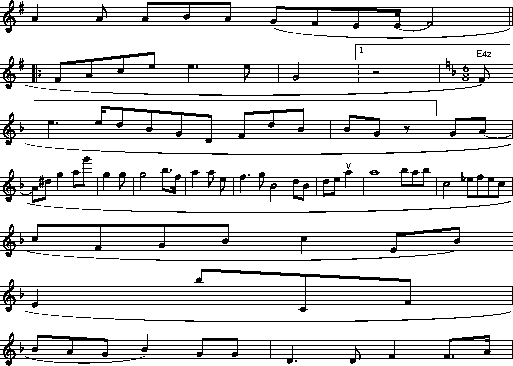
\includegraphics[width=\textwidth]{pics/generated_music_t1_1.png}
\caption{Generated sample 1 with Temperature = 1}
\end{minipage}\hfill
\begin{minipage}{0.48\textwidth}
\centering
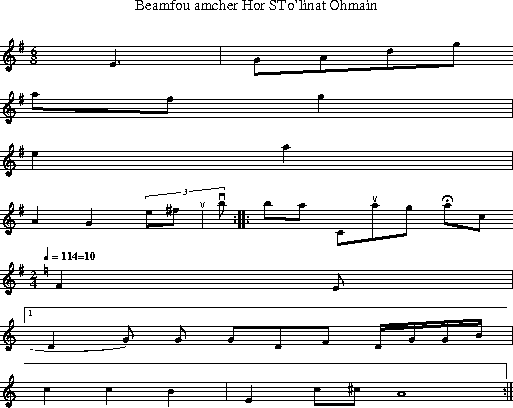
\includegraphics[width=\textwidth]{pics/generated_music_t1_2.png}
\caption{Generated sample 2 with Temperature = 1}
\end{minipage}
\end{figure}
\newpage

\subsubsection{Greater Temperature}
We try setting temperature to be 1.5, pick up the one that makes the most sense, and obtain the following
\begin{lstlisting}
X:8
T:ByE6sie
W:Ava Cosiatisse
TAitenyas Selt ton'agl>a?
R:iein's Crau
R:dung
C:QOun
O:Beecc,a0 a
Be^g dB | c6]0E4 | E4D4F,q E,DE ,> :G2 F,3AG | d3d cBGB^ceg2|a8g2e2 | fd !doa"bs
V:1
Gg/b)gr# "D7Bd^c cB GB "A4ed |
?, j"ptan
L:11,
E F>Ac |
g2e2 
[B2eAGF G4|E3GB2D2!
xds
n:dwnai,>Id setdnyle Che
C:triipe eEaw| 
K:Emiz3E |
E4 _G2DA B_GG :|
g2ge>e g2 | fedeg | bd, O8  b"A,> (3)3FE GGF) | EDEF e:|4 D3ABBAFz2 | (37|D2F6
G4A2|BG=fgfed2 AAAcdA |
">=t4\
A2A,4A,a fga2 |bogga |
ab2g2ec EDDFDD EDe | DHE2 G3D | G2D  E3 (67)B3(G4^G2F|DG)":|: FDF1d2 | e2d2ce |
A2dff2ec BcBAEDBGA2 |2 c,F2AFAGGB :|2 2BcAA |
d_E2 G>dBE2z E,,b2|
|:|
\end{lstlisting}

Moreover, we set the temperature to be 2. The results just don't make anysense
\begin{lstlisting}
dA=BA4|
=}Bd|f4 ggdu | e6B2fBGTc2GE EED|G1t2 AABB |:FEGBA1 \{G4 CE0. e|5E1t L1EA:-zboX
Id Ghte
Nordk ittid
O:-urtanc Aiaboa(#41.=C.ca#,srserc.).S OBanou'c, 
Z:5narur"i Mialresovgle:un At5
M:6/8
K:)
B-2F2e2 W G3z MBd>2)c2A,^F<A,p we]nonh.ap
Z:iic'aj'm Fallz?D's'dB0Odr
n:
F:Pravisieium#9300 KOEkD).
i:n (Divs.m1'tor " Oscavia-w'~Co ey coi
T:Mratil , Id pone'rzhonndouey,41te
R:Mrlathal/
Z:.anBe'R DesBgelcion g?utsoy-1/9
H:OnFr e'Hak D90iiv2~c2eo:wr ptl
BOs Shoc2 Haviermiborodenrsase
C AA^CO )tar 0E, F2nmo. 23ifahndtmotlnicl oaigc2-24 w
EAEx |A2ede2 | Bm VB
e2|Af g)fd e>e/A/ ^HAB>B/c:|B ^k2b/7ued>^G)G+Af^cA2A FEE ]cGFF | Adc edBAm Z|:m
EF]^AG.TBx4 | g6B>EG0|d=c2A>2G |m4(J2ee4f'4>{^c63  Vctc0yuH Ecin-MiSpanc
Dpto+s.fr'Blwgagu"y
\end{lstlisting}
\newpage

\subsection{Discussion}
As is observed from the result above, as temperature goes up, the music becomes more "improvising"  and "creative." When temperature is 0.5, the music follows some potential strict rule like A2 is followed by G2 and then A2 and so forth. It just keeps repeating itself. The lack of variation makes all the music generated highly similar, and the tune headers also make sense. When temperature is 1, the music starts to improvise. It has some variation throughout the text while maintaining some repetition between small sequences. When the temperature gets higher, for example like 1.5, the music becomes some mysterious chaos and the tune header is no more intelligible. When it comes to 2, it can't even follow the format such that no music can be produced at this point.

This pattern can be explained with the formula of softmax with temperature. 
\begin{equation}
softmax(j) = \frac{e^{a_j/T}}{\sum_{i} e^{a_i/T}}
\end{equation}

When we increase T, the curve of softmax becomes smooth, that is, each component of the softmax scales down so that the one which originally has higher portion/probability now does not has much difference from others. Therefore, when we sample the output, the originally highly voted letter has a lower chance to be selected compare with the original case. In this way, the music generation process has more random and improved output letters than the one with lower T. 


\subsection{Hyper Parameters and Model Details}
We design our model as follows.
\begin{figure}[h]
\centering
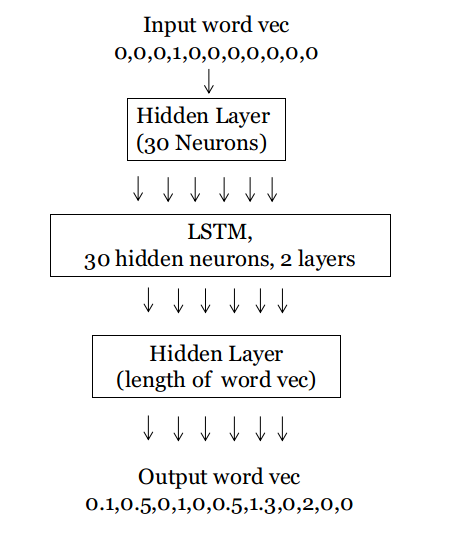
\includegraphics[scale=0.5]{pics/model.png}
\caption{Network structure of our model}
\end{figure}
Our model takes a vector input, which is a one hot representation of a character. It is fed to the first hidden layer of 30 neurons to extract the feature of the word vec. Then it is fed to the LSTM cell. After that it is connected to another hidden layer to convert it in the lenght of the word vec, where it produces a output as a score for each character in the word vec. It is then passed to the softmax layer to convert the score to the probability.

For other hyper parameters, we use learning rate as 0.001, with a scheduler reducing the rate by half every 5 steps.
\newpage
\section{Plots}
\subsection{Training and Validation Plots}
\begin{figure}[h]
\begin{minipage}{0.48\textwidth}
\centering
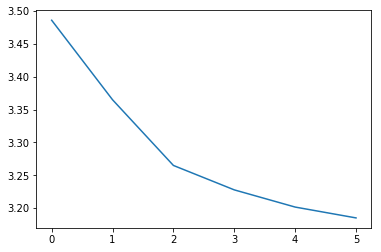
\includegraphics[width=\textwidth]{pics/train_loss_epoch.png}
\caption{Training loss vs. epochs}
\end{minipage}\hfill
\begin{minipage}{0.48\textwidth}
\centering
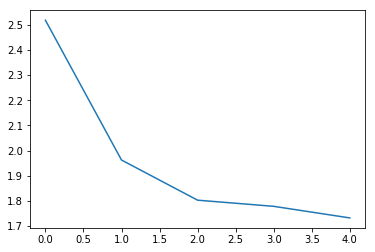
\includegraphics[width=\textwidth]{pics/val_loss_epoch.png}
\caption{Validation loss vs. epochs}
\end{minipage}
\end{figure}

\begin{figure}[h]
\centering
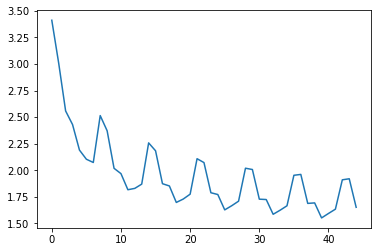
\includegraphics[width=0.7\textwidth]{pics/every_2000_train_loss.png}
\caption{A more detailed training loss: training loss vs. every 2000 chunks of music}
\end{figure}
\subsection{Discussion}
The training and validation loss keeps going down, and it will continue going down if more time is available. Also we can observe that there is some up and down inside one epoch, which has a repeating pattern between epochs. We can conclude that variation of loss is due to some specific music sequences.  
\newpage


\section{Hidden Units}
\subsection{Plots}
\subsection{Discussion}

\section{Dropout}

\section{Optimizer Exploration}

\section{Feature Evaluation}

\section{Contributions}



\section{References}
[1] Bishop, C. M., {\it Neural networks for pattern recognition}, Oxford: Oxford University Press, 2013. \\



\end{document}